\section{变分方程}
\label{sec:odesens-variational}

Gronwall估计只回答“差多少”，不回答“往哪边差”，得到的常数也往往偏大。若解关于数据可微，初值沿某方向变一点时，解的变化就可以用一个线性方程精确算到一阶。这需要先弄清楚解什么时候可微。

\paragraph{连续依赖不能推出可微依赖}
方程$\dot{x}=\lvert x\rvert$的右端全局Lipschitz，$L=1$，解对初值Lipschitz依赖。可是$x_0>0$时解是$x_0\mathrm{e}^{t}$，$x_0<0$时解是$x_0\mathrm{e}^{-t}$，所以
\[
 \varphi_1(x_0)=\begin{cases}\mathrm{e}\,x_0,&x_0\geq0,\\x_0/\mathrm{e},&x_0<0.\end{cases}
\]
$\varphi_1$在$x_0=0$处左导数为$1/\mathrm{e}$，右导数为$\mathrm{e}$，不可微，见图~\ref{fig:odesens-kink}。Lipschitz依赖只限制了差商的大小，并不保证差商有极限。要谈导数，右端本身要可微。

\begin{BookInlineFigure}
  \centering
  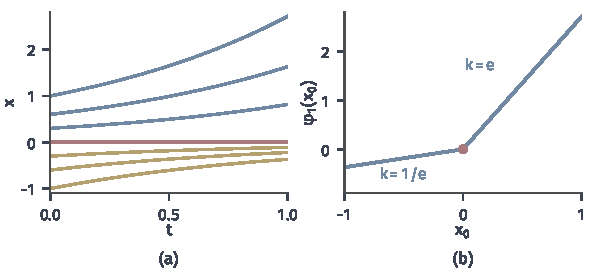
\includegraphics[width=100mm]{figures/06-differential-equations/01-ordinary-differential-equations/matplotlib/odesens-kink/figure.pdf}
  \caption{Lipschitz依赖而不可微。(a)$\dot{x}=\lvert x\rvert$的解：正初值（蓝）按$\mathrm{e}^{t}$增长，负初值（黄）按$\mathrm{e}^{-t}$衰减，红线是零解。(b)$t=1$时的解映射，在红点$x_0=0$处有折点，左右斜率分别为$1/\mathrm{e}$与$\mathrm{e}$。}
  \label{fig:odesens-kink}
\end{BookInlineFigure}

\paragraph{形式推导}
先假设可以求导，看导数应当满足什么方程。设$\bm{x}(t;\bm{x}_0,\bm{\theta})$解
\[
 \dot{\bm{x}}=\bm{f}(t,\bm{x},\bm{\theta}),\qquad \bm{x}(t_0)=\bm{x}_0,
\]
参考解记为$\bm{x}(t)$。沿方向$(\bm{v},\bm{w})$扰动，考虑$\bm{x}(t;\bm{x}_0+\varepsilon\bm{v},\bm{\theta}+\varepsilon\bm{w})$。把积分方程对$\varepsilon$在$0$处求导，记$\bm{z}(t)$为解的方向导数，由链式法则，
\[
 \bm{z}(t)=\bm{v}+\int_{t_0}^{t}\bigl[\bm{A}(s)\bm{z}(s)+\bm{B}(s)\bm{w}\bigr]\,\mathrm{d}s,
\]
其中两个系数沿参考解取值：
\begin{equation}
 \bm{A}(t)=\partial_{\bm{x}}\bm{f}\bigl(t,\bm{x}(t),\bm{\theta}\bigr),\qquad
 \bm{B}(t)=\partial_{\bm{\theta}}\bm{f}\bigl(t,\bm{x}(t),\bm{\theta}\bigr).
 \label{eq:odesens-coefficients}
\end{equation}
这就是
\begin{equation}
 \dot{\bm{z}}=\bm{A}(t)\bm{z}+\bm{B}(t)\bm{w},\qquad \bm{z}(t_0)=\bm{v},
 \label{eq:odesens-variational}
\end{equation}
称为沿参考解的\term{变分方程}（variational equation）。

原方程是非线性的，变分方程却是线性的，系数是沿已知轨迹取值的时变矩阵，第~\ref{chap:linear-differential-systems}章的工具全部可用。上面的推导把求导和积分交换了，也默认了导数存在，下面的定理补上这两点。

\begin{theorem}[解的可微依赖]
\label{thm:odesens-differentiable}
设$\bm{U}\subseteq\mathbb{R}^{n}$、$\bm{\Theta}\subseteq\mathbb{R}^{p}$是开集，取值于$\mathbb{R}^{n}$的右端$\bm{f}$定义在$[t_0,T]\times\bm{U}\times\bm{\Theta}$上，满足：对固定的$(\bm{a},\bm{\theta})$关于$t$可测；对几乎每个$t$，关于$(\bm{a},\bm{\theta})$连续可微。设$\bm{x}:[t_0,T]\to\bm{U}$是参数$\bm{\theta}$、初值$\bm{x}_0$的绝对连续解，并设存在$\rho>0$与可积函数$m\geq0$，使闭管道$\lVert\bm{a}-\bm{x}(t)\rVert_2\leq\rho$落在$\bm{U}$内，闭球$\lVert\bm{\vartheta}-\bm{\theta}\rVert_2\leq\rho$落在$\bm{\Theta}$内，且在其上对几乎每个$t$有
\begin{equation}
 \lVert\partial_{\bm{x}}\bm{f}(t,\bm{a},\bm{\vartheta})\rVert_2\leq m(t),\qquad
 \lVert\partial_{\bm{\theta}}\bm{f}(t,\bm{a},\bm{\vartheta})\rVert_2\leq m(t).
 \label{eq:odesens-derivative-bound}
\end{equation}
则存在$\delta>0$，当$\lVert\bm{v}\rVert_2+\lVert\bm{w}\rVert_2<\delta$时，初值$\bm{x}_0+\bm{v}$、参数$\bm{\theta}+\bm{w}$的解$\bm{y}$在$[t_0,T]$上存在且唯一，并且
\begin{equation}
 \sup_{t\in[t_0,T]}\bigl\lVert\bm{y}(t)-\bm{x}(t)-\bm{z}(t)\bigr\rVert_2=o\bigl(\lVert\bm{v}\rVert_2+\lVert\bm{w}\rVert_2\bigr),
 \label{eq:odesens-differentiable}
\end{equation}
其中$\bm{z}$是变分方程~\eqref{eq:odesens-variational}的解。
\end{theorem}

\begin{proof}
记扰动的大小为
\[
 \lVert\bm{\eta}\rVert=\lVert\bm{v}\rVert_2+\lVert\bm{w}\rVert_2,
\]
并记$M=\int_{t_0}^{T}m$。

\emph{第一步，解的存在与线性控制。}由式~\eqref{eq:odesens-derivative-bound}和中值不等式，右端在管道内关于状态有Lipschitz系数$m(t)$，关于参数有系数$m(t)$。按定理~\ref{thm:odesens-local-lipschitz}的管道论证，把常数$L$换成可积系数$m(t)$，并使用第~\ref{chap:ode-existence-continuation}章Carathéodory情形的延拓结论，只要$\delta$足够小，$\bm{y}$就在$[t_0,T]$上存在并留在管道内。由式~\eqref{eq:odesens-perturbation-bound}，取残差$\varepsilon\leq m\lVert\bm{w}\rVert_2$，
\[
 \lVert\bm{y}(t)-\bm{x}(t)\rVert_2\leq\mathrm{e}^{M}\lVert\bm{v}\rVert_2+M\mathrm{e}^{M}\lVert\bm{w}\rVert_2\leq C\lVert\bm{\eta}\rVert,
\]
其中$C=(1+M)\mathrm{e}^{M}$。

\emph{第二步，写出余项的方程。}记$\bm{\Delta}=\bm{y}-\bm{x}$，$\bm{R}=\bm{\Delta}-\bm{z}$，则$\bm{R}(t_0)=\bm{0}$。对几乎每个固定的$t$，沿线段$\sigma\mapsto(\bm{x}+\sigma\bm{\Delta},\bm{\theta}+\sigma\bm{w})$用微积分基本定理，
\[
 \bm{f}(t,\bm{y},\bm{\theta}+\bm{w})-\bm{f}(t,\bm{x},\bm{\theta})
 =\int_0^1\bigl[\partial_{\bm{x}}\bm{f}^{\sigma}\,\bm{\Delta}+\partial_{\bm{\theta}}\bm{f}^{\sigma}\,\bm{w}\bigr]\,\mathrm{d}\sigma,
\]
$\partial\bm{f}^{\sigma}$表示在线段上$\sigma$处取值。减去$\bm{A}\bm{z}+\bm{B}\bm{w}$，得到
\[
 \dot{\bm{R}}=\bm{A}\bm{R}+\bm{E},\qquad
 \bm{E}(t)=\int_0^1\bigl[(\partial_{\bm{x}}\bm{f}^{\sigma}-\bm{A})\bm{\Delta}+(\partial_{\bm{\theta}}\bm{f}^{\sigma}-\bm{B})\bm{w}\bigr]\,\mathrm{d}\sigma.
\]

\emph{第三步，估计$\bm{E}$。}定义
\[
 \omega_{\bm{\eta}}(t)=\sup\bigl(\lVert\partial_{\bm{x}}\bm{f}(t,\bm{a},\bm{\vartheta})-\bm{A}(t)\rVert_2+\lVert\partial_{\bm{\theta}}\bm{f}(t,\bm{a},\bm{\vartheta})-\bm{B}(t)\rVert_2\bigr),
\]
上确界取遍满足下式的$(\bm{a},\bm{\vartheta})$：
\[
 \lVert\bm{a}-\bm{x}(t)\rVert_2\leq C\lVert\bm{\eta}\rVert,\qquad\lVert\bm{\vartheta}-\bm{\theta}\rVert_2\leq\lVert\bm{\eta}\rVert.
\]
被取上确界的量关于$(\bm{a},\bm{\vartheta})$连续，上确界可以改取可数稠密子集，所以$\omega_{\bm{\eta}}$可测。由第一步，
\[
 \lVert\bm{E}(t)\rVert_2\leq\omega_{\bm{\eta}}(t)\bigl(\lVert\bm{\Delta}(t)\rVert_2+\lVert\bm{w}\rVert_2\bigr)\leq(C+1)\lVert\bm{\eta}\rVert\,\omega_{\bm{\eta}}(t).
\]

\emph{第四步，取极限。}对$\dot{\bm{R}}=\bm{A}\bm{R}+\bm{E}$取积分形式与范数，得到
\[
 \lVert\bm{R}(t)\rVert_2\leq\int_{t_0}^{t}\bigl(m\lVert\bm{R}\rVert_2+\lVert\bm{E}\rVert_2\bigr)\,\mathrm{d}s.
\]
由引理~\ref{lem:odesens-gronwall}，
\[
 \sup_{t}\lVert\bm{R}(t)\rVert_2\leq\mathrm{e}^{M}(C+1)\lVert\bm{\eta}\rVert\int_{t_0}^{T}\omega_{\bm{\eta}}(s)\,\mathrm{d}s.
\]
当$\lVert\bm{\eta}\rVert\to0$时，由导数对$(\bm{a},\bm{\vartheta})$的连续性，$\omega_{\bm{\eta}}\to0$几乎处处成立；又$\omega_{\bm{\eta}}\leq4m$可积。控制收敛定理给出$\int\omega_{\bm{\eta}}\to0$，这就是式~\eqref{eq:odesens-differentiable}。
\end{proof}

定理的条件各有分工。对状态和参数连续可微，保证了第三步的$\omega_{\bm{\eta}}\to0$，把它换成Lipschitz就会出现$\lvert x\rvert$那样的折点。统一的可积上界$m$既给出第一步的管道，也提供控制收敛定理所需的控制函数。对时间只要求可测，所以$\bm{A}$、$\bm{B}$可以在输入切换的时刻跳变，变分方程几乎处处成立。

对$\bm{v},\bm{w}$而言，$\bm{z}$是线性的，所以式~\eqref{eq:odesens-differentiable}说的正是解映射在该点Fréchet可微。把参考点也变动，$\bm{A}$、$\bm{B}$按$L^1$连续变化（同样由控制收敛定理），线性方程的解也随之连续变化，因此解映射是连续可微的。这里所有结论只针对给定解的管道内。

\paragraph{一阶预测与余项}
变分方程给出一阶预测$\bm{y}\approx\bm{x}+\bm{z}$。余项$o(\cdot)$说明小扰动下预测越来越准，但没有说多小才算小。若导数本身Lipschitz，余项可以写出来。

\begin{theorem}[一阶预测的余项]
\label{thm:odesens-remainder}
在定理~\ref{thm:odesens-differentiable}的设定中，只改变初值（$\bm{w}=\bm{0}$），设$\bm{y}$与$\bm{x}$之间的线段留在管道内，$\lVert\partial_{\bm{x}}\bm{f}\rVert_2\leq L$，且$\partial_{\bm{x}}\bm{f}$关于状态有Lipschitz常数$M_2$，$L>0$。则
\begin{equation}
 \lVert\bm{y}(t)-\bm{x}(t)-\bm{z}(t)\rVert_2\leq\frac{M_2}{2}\,\lVert\bm{v}\rVert_2^2\,\frac{\mathrm{e}^{L(t-t_0)}\bigl(\mathrm{e}^{L(t-t_0)}-1\bigr)}{L}.
 \label{eq:odesens-remainder}
\end{equation}
\end{theorem}

\begin{proof}
沿用上一定理第二步的记号，$\bm{w}=\bm{0}$。线段上$\sigma$处的$\partial_{\bm{x}}\bm{f}$与$\bm{A}$相差不超过$M_2\sigma\lVert\bm{\Delta}\rVert_2$，所以
\[
 \lVert\bm{E}(s)\rVert_2\leq\int_0^1M_2\sigma\,\mathrm{d}\sigma\,\lVert\bm{\Delta}(s)\rVert_2^2=\frac{M_2}{2}\lVert\bm{\Delta}(s)\rVert_2^2.
\]

由式~\eqref{eq:odesens-basic-estimate}，有
\[
 \lVert\bm{\Delta}(s)\rVert_2\leq\mathrm{e}^{L(s-t_0)}\lVert\bm{v}\rVert_2.
\]
再对$\dot{\bm{R}}=\bm{A}\bm{R}+\bm{E}$用同一估计，得到
\[
 \lVert\bm{R}(t)\rVert_2\leq\frac{M_2}{2}\lVert\bm{v}\rVert_2^2\int_{t_0}^{t}\mathrm{e}^{L(t-s)}\mathrm{e}^{2L(s-t_0)}\,\mathrm{d}s.
\]
积分等于$\mathrm{e}^{L(t-t_0)}\bigl(\mathrm{e}^{L(t-t_0)}-1\bigr)/L$，结论成立。
\end{proof}

\begin{example}[Logistic方程的一阶预测]
\label{ex:odesens-first-order}
继续$\dot{x}=x(1-x)$，$x_0=1/4$，$T=\ln3$，已知$x(T)=1/2$。沿解$A(t)=1-2x(t)$，变分方程$\dot{z}=A(t)z$的解是
\[
 z(T)=v\,\exp\int_0^T\bigl(1-2x(t)\bigr)\,\mathrm{d}t.
\]

把积分变量换成$x$，用$\mathrm{d}t=\mathrm{d}x/(x(1-x))$，得到
\[
 \int_0^T(1-2x)\,\mathrm{d}t=\int_{1/4}^{1/2}\frac{1-2x}{x(1-x)}\,\mathrm{d}x=\Bigl[\ln x(1-x)\Bigr]_{1/4}^{1/2}=\ln\frac43.
\]
所以$z(T)=\tfrac43v$，一阶预测是$y(T)\approx\tfrac12+\tfrac43v$。

用解析解验证。$v=0.1$时$y_0=0.35$，真实值$0.6176$，预测值$0.6333$，余项$-0.0157$；$v=-0.1$时$y_0=0.15$，真实值$0.3462$，预测值$0.3667$，余项$-0.0205$。

这里$M_2=\sup\lvert f''\rvert=2$，$L=1$，式~\eqref{eq:odesens-remainder}给出余项不超过$\mathrm{e}^{T}(\mathrm{e}^{T}-1)v^2=6v^2$，$v=\pm0.1$时为$0.06$，确实盖住了真实余项。
\end{example}

图~\ref{fig:odesens-first-order}(a)显示，预测线是真实曲线在$y_0=1/4$处的切线，$y_0$稍远就分开。$y_0=0.7$时预测值$1.1$超出了状态可能的范围$[0,1]$，而真实值是$0.875$。(b)的对数坐标中余项的斜率是$2$，正是一阶预测的误差量级。

\begin{BookInlineFigure}
  \centering
  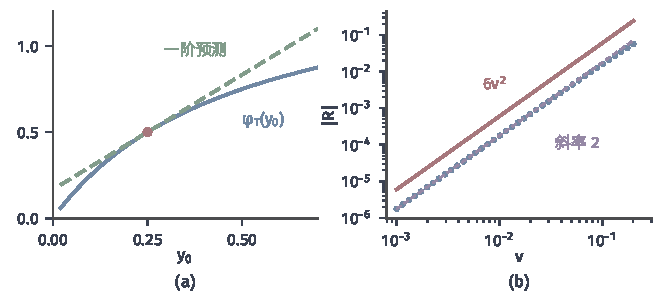
\includegraphics[width=112mm]{figures/06-differential-equations/01-ordinary-differential-equations/matplotlib/odesens-first-order/figure.pdf}
  \caption{Logistic方程的一阶预测，$T=\ln3$。(a)解映射$\varphi_T$（蓝）与红点处的一阶预测$\tfrac12+\tfrac43(y_0-\tfrac14)$（绿虚线）。(b)余项$\lvert R\rvert$随$v$的变化（蓝点），红线是上界$6v^2$，紫色虚线是斜率为$2$的参考线。}
  \label{fig:odesens-first-order}
\end{BookInlineFigure}

\subsection{初值导数}
\label{sec:odesens-initial-derivative}

只改变初值时$\bm{w}=\bm{0}$，变分方程齐次，解对$\bm{v}$线性。把$\bm{v}$依次取为$\mathbb{R}^{n}$的标准基，所得$n$个解排成一个矩阵，也就是解对初始状态的Jacobian矩阵
\begin{equation}
 \bm{S}(t)=\frac{\partial\bm{x}(t;\bm{x}_0)}{\partial\bm{x}_0}\in\mathbb{R}^{n\times n}.
 \label{eq:odesens-initial-jacobian}
\end{equation}
由式~\eqref{eq:odesens-variational}，它满足以单位矩阵为初值的线性系统
\begin{equation}
 \dot{\bm{S}}=\bm{A}(t)\bm{S},\qquad \bm{S}(t_0)=\bm{I}.
 \label{eq:odesens-initial-variational}
\end{equation}

这正是第~\ref{chap:linear-differential-systems}章的状态转移矩阵的定义方程。那里证明了$\bm{\Phi}(t,s)$对$t$满足该线性系统、$\bm{\Phi}(s,s)=\bm{I}$，并满足复合关系$\bm{\Phi}(t,s)\bm{\Phi}(s,r)=\bm{\Phi}(t,r)$。因此$\bm{S}(t)=\bm{\Phi}(t,t_0)$，只是这里的$\bm{A}(t)$来自沿解的线性化，$\bm{\Phi}$依赖于所选的轨迹。

\paragraph{水面上的小木棍}
想象在水流中放一根极短的小木棍，一端在参考点$\bm{x}_0$，另一端在$\bm{x}_0+\bm{v}$。水流带着小木棍前进，同时拉长、压短并转动它。$\bm{z}(t)=\bm{S}(t)\bm{v}$就是$t$时刻的小木棍。对应关系是：水流是右端$\bm{f}$，小木棍是切向量，$\bm{A}(t)$描述当前位置附近水流的局部拉伸与旋转。类比到有限长度就失效了，长木棍会弯曲，而$\bm{z}$永远是直的箭头。

把$\bm{S}(t)$作奇异值分解$\bm{S}=\bm{U}\bm{\Sigma}\bm{V}^{\top}$。单位球面上的初值方向被映成椭球面，最大奇异值$\sigma_{\max}$是一阶下最坏的放大倍数，相应的$\bm{V}$的列是最敏感的初值方向，$\bm{U}$的列是响应的方向。

\begin{example}[可以手算的二维系统]
\label{ex:odesens-planar}
考虑
\[
 \dot{x}_1=-x_1,\qquad \dot{x}_2=x_2+x_1^2,
\]
初值$(1,0)$。第一个方程给出$x_1(t)=\mathrm{e}^{-t}$，沿解的线性化系数是
\[
 \bm{A}(t)=\begin{bmatrix}-1&0\\2\mathrm{e}^{-t}&1\end{bmatrix}.
\]

按列解式~\eqref{eq:odesens-initial-variational}。第二列满足$\dot{s}_{1,2}=-s_{1,2}$、$\dot{s}_{2,2}=2\mathrm{e}^{-t}s_{1,2}+s_{2,2}$，初值$(0,1)$，于是
\[
 s_{1,2}=0,\qquad s_{2,2}=\mathrm{e}^{t}.
\]
第一列初值为$(1,0)$，由第一个方程得$s_{1,1}=\mathrm{e}^{-t}$，代入第二个方程，
\[
 \dot{s}_{2,1}=s_{2,1}+2\mathrm{e}^{-2t},\qquad s_{2,1}(0)=0.
\]

乘以积分因子$\mathrm{e}^{-t}$，得
\[
 \frac{\mathrm{d}}{\mathrm{d}t}\bigl(\mathrm{e}^{-t}s_{2,1}\bigr)=2\mathrm{e}^{-3t},
\]
积分后得到
\[
 s_{2,1}(t)=\tfrac23\bigl(\mathrm{e}^{t}-\mathrm{e}^{-2t}\bigr).
\]
取$t=\ln2$，参考解到达$(1/2,\,7/12)$，
\[
 \bm{S}(\ln2)=\begin{bmatrix}1/2&0\\7/6&2\end{bmatrix}.
\]

这个方程能显式求解，可以用来核对：从$(a,b)$出发，
\[
 x_1=a\mathrm{e}^{-t},\qquad x_2=\bigl(b+a^2/3\bigr)\mathrm{e}^{t}-\bigl(a^2/3\bigr)\mathrm{e}^{-2t}.
\]
对$(a,b)$在$(1,0)$处求导，结果与上式相同。$\bm{S}(\ln2)$的奇异值是$2.330$与$0.429$，最大奇异值比特征值$2$更大，这个差别来自$\bm{S}$非对称带来的转向。
\end{example}

图~\ref{fig:odesens-tangent-transport}把例~\ref{ex:odesens-planar}画了出来。红色小圆的两根基向量被$\bm{S}(\ln2)$带到蓝色箭头：$(1,0)$方向既缩短又转向，$(0,1)$方向被拉长两倍。半径$0.4$并不算小，真实的像（蓝色区域）和线性预测的椭圆（绿色虚线）已有肉眼可见的差别。

\begin{BookInlineFigure}
  \centering
  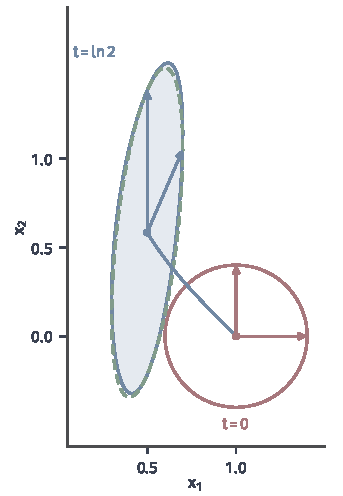
\includegraphics[width=58mm]{figures/06-differential-equations/01-ordinary-differential-equations/matplotlib/odesens-tangent-transport/figure.pdf}
  \caption{小圆随流的变形。方程为$\dot{x}_1=-x_1$，$\dot{x}_2=x_2+x_1^2$。红圆是$t=0$时以$(1,0)$为心、半径$0.4$的圆，蓝线是圆心的轨迹，浅蓝区域是$t=\ln2$时圆的真实像，绿色虚线是线性预测$\bm{x}(t)+\bm{S}(t)\bm{v}$的椭圆。红箭头是两根基向量，蓝箭头是它们在$\bm{S}(\ln2)$下的像。}
  \label{fig:odesens-tangent-transport}
\end{BookInlineFigure}

\paragraph{沿轨迹方向的导数}
自治方程有一个不用解方程就知道的解。对$\bm{f}(\bm{x}(t))$关于$t$求导，并用$\dot{\bm{x}}=\bm{f}(\bm{x})$，得到
\[
 \frac{\mathrm{d}}{\mathrm{d}t}\bm{f}(\bm{x}(t))=\bm{A}(t)\bm{f}(\bm{x}(t)).
\]
所以$\bm{f}(\bm{x}(t))$满足齐次变分方程，初值是$\bm{f}(\bm{x}_0)$。由线性方程的唯一性，
\begin{equation}
 \bm{S}(t)\,\bm{f}(\bm{x}_0)=\bm{f}(\bm{x}(t)).
 \label{eq:odesens-tangent-flow}
\end{equation}
含义是：把初值沿轨迹挪一点，只相当于把时间起点平移，$t$时刻的解也沿轨迹挪一点。

标量情形下，当$f(x_0)\neq0$时，式~\eqref{eq:odesens-tangent-flow}直接给出$S(t)=f(x(t))/f(x_0)$。在Logistic方程上，
\[
 S(\ln3)=\frac{\tfrac12\cdot\tfrac12}{\tfrac14\cdot\tfrac34}=\frac43,
\]
与例~\ref{ex:odesens-first-order}的积分结果一致。再继续到$t=2\ln3$，$x$从$1/2$增长到$3/4$，这一段的放大倍数是$(3/16)/(1/4)=3/4$，全程是$\tfrac43\cdot\tfrac34=1$，放大和压缩恰好抵消，这正是复合关系$\bm{\Phi}(t,s)\bm{\Phi}(s,r)=\bm{\Phi}(t,r)$的一个实例。

\paragraph{增长的$\bm{S}$不等于发散的轨迹}
Jacobian矩阵增长并不说明解跑远了。无阻尼摆$\dot{q}=p$、$\dot{p}=-\sin q$的轨道是封闭曲线，但周期依赖振幅。两条相邻轨道相位差随时间线性累积，$\bm{S}$的范数因而线性增长，见图~\ref{fig:odesens-pendulum-growth}。这里的增长来自相位的错开，不是轨道的分离，而轨迹全程有界。这再次说明，有限时间的一阶响应和长期行为是不同的问题。

\begin{BookInlineFigure}
  \centering
  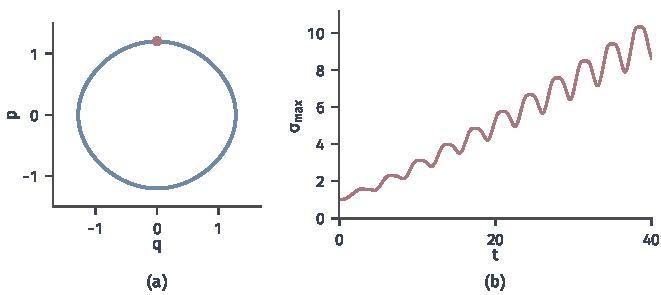
\includegraphics[width=112mm]{figures/06-differential-equations/01-ordinary-differential-equations/matplotlib/odesens-pendulum-growth/figure.pdf}
  \caption{无阻尼摆的初值Jacobian矩阵。(a)从红点$(q,p)=(0,1.2)$出发的封闭轨道。(b)式~\eqref{eq:odesens-initial-variational}数值积分得到的最大奇异值$\sigma_{\max}(t)$，在振荡中近似线性增长，$t=40$内从$1$升到约$10$，而轨道始终有界。}
  \label{fig:odesens-pendulum-growth}
\end{BookInlineFigure}

\subsection{参数导数}
\label{sec:odesens-parameter-derivative}

现在让参数变化。先取有限维参数$\bm{\theta}\in\mathbb{R}^{p}$，初值也可能依赖参数，写成$\bm{x}_0(\bm{\theta})$。把$\bm{w}$取遍标准基，方向导数排成矩阵
\begin{equation}
 \bm{P}(t)=\frac{\partial\bm{x}(t;\bm{\theta})}{\partial\bm{\theta}}\in\mathbb{R}^{n\times p}.
 \label{eq:odesens-parameter-jacobian}
\end{equation}
在式~\eqref{eq:odesens-variational}中$\bm{v}=(\partial_{\bm{\theta}}\bm{x}_0)\bm{w}$，于是$\bm{P}$满足
\begin{equation}
 \dot{\bm{P}}=\bm{A}(t)\bm{P}+\bm{B}(t),\qquad \bm{P}(t_0)=\partial_{\bm{\theta}}\bm{x}_0(\bm{\theta}).
 \label{eq:odesens-parameter-variational}
\end{equation}
与初值导数相比，多了非齐次项$\bm{B}(t)$：参数改变时，每一时刻的变化率都被额外推了一下。

这个线性方程的解由第~\ref{chap:linear-differential-systems}章的常数变易公式给出：
\begin{equation}
 \bm{P}(t)=\bm{\Phi}(t,t_0)\,\partial_{\bm{\theta}}\bm{x}_0+\int_{t_0}^{t}\bm{\Phi}(t,s)\bm{B}(s)\,\mathrm{d}s.
 \label{eq:odesens-parameter-formula}
\end{equation}
第一项是初值本身对参数的依赖，第二项是时刻$s$对变化率的推动再传播到$t$。结构和Gronwall上界完全对应，只是把放大因子的上界换成了真实的传播矩阵。

\begin{example}[增长率的导数]
\label{ex:odesens-parameter-derivative}
对$\dot{x}=\theta x(1-x)$，$\theta=1$，$x_0=1/4$，系数是
\[
 A(t)=1-2x(t),\qquad B(t)=x(t)(1-x(t)).
\]
初值不依赖参数，所以$P(0)=0$。式~\eqref{eq:odesens-parameter-variational}是$\dot{P}=(1-2x)P+x(1-x)$。

猜测$P=t\,x(1-x)$，即$P=tf(x)$，代入验证。由$\frac{\mathrm{d}}{\mathrm{d}t}f(x)=(1-2x)f(x)$，得到
\[
 \dot{P}=f(x)+t(1-2x)f(x)=x(1-x)+(1-2x)P,
\]
满足方程，且$P(0)=0$。这个结果也可以这样理解：解依赖$\theta t$，改变$\theta$相当于改变时间尺度。

在$t=\ln3$处，$x=1/2$，$P(\ln3)=\tfrac14\ln3\approx0.2747$。$\theta$增加$0.2$时，一阶预测的改变量是$0.0549$，例~\ref{ex:odesens-parameter-bound}中的真实差是$0.0547$，而Gronwall上界是$0.0901$。

若初值也依赖参数，比如$x_0(\theta)=\theta/4$，则$\partial_\theta x_0=1/4$，由式~\eqref{eq:odesens-parameter-formula}，
\[
 P(\ln3)=\frac43\cdot\frac14+\frac14\ln3\approx0.3333+0.2747=0.6080.
\]
前一项用了初值导数$S(\ln3)=4/3$。
\end{example}

图~\ref{fig:odesens-parameter-derivative}画出了$P(t)$。参数的影响在$x$中等时最大，$x$接近$0$或$1$时增长率的具体数值几乎不起作用。绿点是有限差分，它与变分方程的解重合。

\begin{BookInlineFigure}
  \centering
  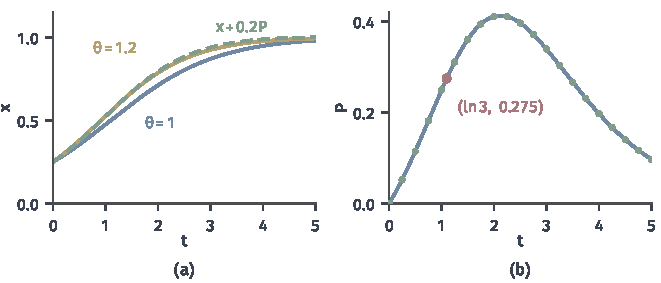
\includegraphics[width=112mm]{figures/06-differential-equations/01-ordinary-differential-equations/matplotlib/odesens-parameter-derivative/figure.pdf}
  \caption{参数导数。方程$\dot{x}=\theta x(1-x)$，$x_0=1/4$。(a)$\theta=1$（蓝）、$\theta=1.2$（黄）的解，绿色虚线是一阶预测$x+0.2P$。(b)$P(t)$的变分方程解（蓝）与有限差分（绿点），红点是$t=\ln3$处的值。}
  \label{fig:odesens-parameter-derivative}
\end{BookInlineFigure}

\paragraph{参数化的输入}
输入是一个函数，自由度无穷多。常见的做法是用有限个参数表示它，比如$\bm{g}(t)=\bm{g}(t;\bm{\theta})$，然后归入上面的计算。右端写成$\bm{f}(t,\bm{x},\bm{g}(t;\bm{\theta}))$，由链式法则，
\begin{equation}
 \bm{B}(t)=\partial_{\bm{g}}\bm{f}\bigl(t,\bm{x}(t),\bm{g}(t;\bm{\theta})\bigr)\,\partial_{\bm{\theta}}\bm{g}(t;\bm{\theta}).
 \label{eq:odesens-input-derivative}
\end{equation}
其余不变。定理~\ref{thm:odesens-differentiable}对$t$只要求可测，$\partial_{\bm{\theta}}\bm{g}$可以有跳变。

考虑$\dot{x}=-x+g(t)$，$x_0=0$，$t\in[0,2]$，$g$在$[0,1)$上取$\theta_1$，在$[1,2)$上取$\theta_2$，这里取$\theta_1=1$、$\theta_2=2$。此时$A=-1$，$\bm{B}(t)$在两段上分别是$(1,0)$与$(0,1)$，于是$P_j$分别解$\dot{P}_j=-P_j+B_j$。直接积分，
\[
 P_1(2)=\mathrm{e}^{-1}(1-\mathrm{e}^{-1})\approx0.2325,\qquad
 P_2(2)=1-\mathrm{e}^{-1}\approx0.6321.
\]
较早的输入经历了$\mathrm{e}^{-1}$的衰减，对末态的影响较小，图~\ref{fig:odesens-input-basis}(b)的折点就发生在切换时刻。

\begin{BookInlineFigure}
  \centering
  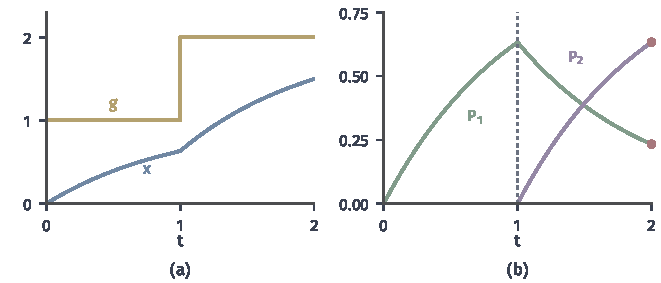
\includegraphics[width=112mm]{figures/06-differential-equations/01-ordinary-differential-equations/matplotlib/odesens-input-basis/figure.pdf}
  \caption{分段常值输入的参数导数。方程$\dot{x}=-x+g$，$x_0=0$。(a)输入$g$（黄）与解$x$（蓝），$\theta=(1,2)$。(b)参数导数$P_1$（绿）、$P_2$（紫），灰色虚线是切换时刻$t=1$，红点是$t=2$时的值。}
  \label{fig:odesens-input-basis}
\end{BookInlineFigure}
